\documentclass[12pt]{book}
\usepackage{booktabs}
\usepackage[table]{xcolor}
\usepackage{tcolorbox}
\usepackage[T1]{fontenc}
\usepackage{wrapfig}
\usepackage{url}
\usepackage{dsfont}
\usepackage{enumitem}
\usepackage{array}
\usepackage{booktabs}

\usepackage{mathtools, nccmath}
\usepackage[polish]{babel}
\usepackage[utf8]{inputenc}
\usepackage{lmodern}
\usepackage{pifont}
\usepackage{blkarray, bigstrut}
\usepackage{amsmath}
\usepackage{kbordermatrix}
\usepackage{cases}
\usepackage{graphicx}
\usepackage{cellspace}
\usepackage[T1]{fontenc}
\usepackage{amsthm}
\selectlanguage{polish}
\usepackage{amsmath}
\usepackage{graphicx}
\usepackage{float}
\usepackage{cite}
\usepackage[margin=2.5cm]{geometry}
\theoremstyle{plain}
\newtheorem{definicja}{Definicja}
\newtheorem{twr}{Twierdzenie}
\newtheorem{lem}[twr]{Lemat}
\newtheorem{mur}{Murphy}[section]
\newcolumntype{P}[1]{>{\centering\arraybackslash}p{#1}}
\newcommand\green{\cellcolor{green!10}}
\newcommand\cincludegraphics[2][]{\raisebox{-0.5\height}{\includegraphics[#1]{#2}}}
\newcommand\red{\cellcolor{red!20}}
\newcommand\blue{\cellcolor{blue!20}}
\newcommand{\R}{\mathbb{R}}
\newcommand*{\tabbox}[2][t]{%
	\vspace{0pt}\parbox[#1][3.7\baselineskip]{1cm}{\strut#2\strut}}
\newcommand\addtag{\refstepcounter{equation}
\renewcommand{\labelenumii}{\theenumii}
\renewcommand{\theenumii}{\theenumi.\arabic{enumii}.}
\tag{\theequation}}

\begin{document}
\title{Optymalizacja  systemu sygnalizacji świetlnej w 
oparciu o przepływowy model ruchu pojazdów.}
\author{Michał Lis}
\date{\today}
\maketitle
\tableofcontents
\chapter{Wprowadzenie}
Problem zatłoczonych ulic staje się coraz bardziej powszechny na całym świecie. W ogromnym tempie wzrasta ilość pojazdów na drogach.
%Problem zatłoczonych ulic staje się coraz bardziej powszechny na całym świecie, głównie ze względu na wzrost ekonomiczny. Według banku światowego w roku 1990 suma produktów krajowych brutto wszystkich państw świata wynosiła 22,6 biliona dolarów \cite{worldBank}. Najbardziej aktualne dane banku światowego dotyczą lat 2012-2017. W czasie ich trwania analogiczna wartość oscylowała wokół 75 bilionów dolarów. Nawet przy uwzględnieniu inflacji dolara, która od w okresie 1990 do 2015 wyniosła $80\%$ światowy produkt brutto jest obecnie prawie dwukrotnie większy w porównaniu do roku 1990. Bezpośrednim skutkiem ogólnoświatowego wzrostu stopy życiowej jest zwiększenie ilości samochodów na drogach.
Według danych firmy gromadzącej dane statystyczne \textit{Statista} liczba zarejestrowanych pojazdów na świecie w roku 2006 wynosiła 947 tysięcy \cite{liczbaPojazdowSwiat}. W 2015 roku na świecie jeździło już 1282 tysięcy pojazdów. Wzrost przez te 9 lat był niemalże liniowy. Co roku rejestrowano około 39,4 tysięcy nowych samochodów rocznie, co wyznacza stopę wzrostu liczby pojazdów na poziomie 3,7$\%$.
\begin{figure}[H]
  \centering
    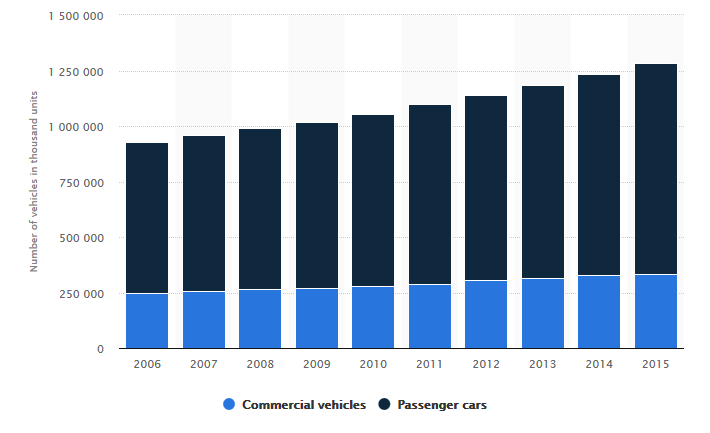
\includegraphics[width=14cm]{liczbaPojazdowSwiat}
 \caption{Liczba pojazdów na świecie}
 \label{fig:liczbaPojazdowSwiat}
\end{figure} \noindent
W Polsce wzrost ilości pojazdów w latach 2006 - 2015 był jeszcze większy \cite{liczbaPojazdowPolska}. W 2006 roku według GUS w Polsce było zarejestrowanych 13,4 miliona samochodów osobowych. W 2015 roku ich liczba wynosiła już 20,7 miliona, co oznacza 5 procentowy roczny wzrost.
Najbardziej zatłoczonym polskim miastem jest Łódź. Według rankingu firmy \textit{TomTom } Łódź zajmuje bardzo wysokie 5 miejsce na świecie i 1 w Europie pod względem zatłoczenia dróg \cite{rankingTomTom}. Oprócz Łodzi w pierwszej setce najbardziej zatłoczonych miast świata są inne polskie miasta: Lublin(34), Kraków(48), Warszawa(50), Wrocław(63), Poznań(69), Bydgoszcz(83). Problem całej Europy. Spośród 100 najbardziej zatłoczonych miast świata aż 45 znajduje się w Europie. W 2008 roku Unia Europejska oszacowała, iż koszty zatłoczenia dróg kształtują się na poziomie $0,9\%-1,5\%$ PKB unijnego \cite{ue2008}. Następny raport z 2017 roku może napawać optymizmem, gdyż przedstawione w nim wyliczenia określiły jedynie $0,77\%$ straty całkowitego PKB wspólnoty \cite{ue2017}. Ten sam raport ocenia koszty zatorów komunikacyjnych w Polsce na poziomie $1,2\%$ polskiego PKB.
Problemy zatorów komunikacyjnych w miastach są o tyle trudniejsze do rozwiązania niż poza miastem, ponieważ na terenach zurbanizowanych brakuje często miejsca na wybudowanie dróg o większej przepustowości. Rozwiązaniem może być wprowadzenie większej ilości sygnalizacji świetlnych. Istotną kwestią jest optymalizacja ustawień sygnalizacji świetlnej. Praca moja jest poświęcona temu problemowi. 
%W celu uzyskania danych potrzebnych do tego procesu rozstawiane są na drogach detektory ruchu. 
%\begin{figure}[H]
%  \centering
%    \includegraphics[width=14cm]{Detektor}
% \caption{System pętli do detekcji osi pojazdów zainstalowany na badawczym stanowisku pomiarowym na drodze DK81 będący w dyspozycji Katedry Metrologii i Elektroniki AGH.}
% \label{fig:Detektor}
%\end{figure} \noindent
%W miastach zachodnioeuropejskich rezultaty naprawdę widać dopiero po roku, gdy system zgromadzi już ogromną ilość danych - mówi Misiorny
%
%Czytaj więcej: https://dzienniklodzki.pl/masz-uwagi-do-sygnalizacji-swietlnej-w-lodzi-wyslij-email-do-zdit/ar/9253440
\chapter{Cel i zakres pracy}
Celem pracy jest stworzenie programu, który zoptymalizuje fazy sygnalizacji świetlnej, co przyczyni się do zwiększenia przepustowości sieci dróg.\\ Jako środowisko zostanie stworzony symulator ruchu drogowego. Symulacje ruchu będą w pełni zgodne z makroskopowym modelem ruchu. Sam makroskopowy model ruchu zostanie przedstawiony w rozdziale X. Jest to model ciągły. Pożądanym jest dyskretny model ruchu drogowego ze względu na łatwość implementacji komputerowej. Zostanie zatem przedstawiona w sekcji X.Y dyskretyzacja makroskopowego modelu ruchu. W rozdziale X zostanie zdefiniowany model sieci dróg. Początkowy model zaplanowano jako podstawowy z pominięciem większości aspektów. W każdej kolejnej sekcji model będzie stopniowo rozwijany. Sieci dróg zdefiniowane według końcowego modelu będą środowiskiem treningowym dla algorytmów uczenia maszynowego. Rozdział X opisuje uczenie ze wzmocnieniem - algorytm treningowy procesu optymalizacji sygnalizacji świetlnej. Rozdział X przedstawia cztery modele sieci dróg, dla których został stworzony program symulacyjny. Rozdział X opisuje optymalizację sygnalizacji świetlnej dla wspomnianych sieci dróg.


   
\chapter{Siatka czasowa i przestrzenna}
Dyskretny charakter modelu przedstawianego w pracy obliguje do określenia siatki czasowej i przestrzennej. Dla par czasu i miejsc należących do tych dwóch siatek będą określane zmienne stanu. \\ \\ \textbf{Siatka czasowa} jest zdefiniowana jako skończony ciąg liczb naturalnych:
\[(0,1,...,K). \addtag \]
Niech będzie ustalona droga $e$, która jest odcinkiem $[0,L_e]$. Droga zostaje podzielona na $L+1$ odcinków o równej długości $\Delta x=\frac{L_e}{L+1}$. \textbf{Siatka przestrzenna} drogi to ciąg odcinków:
\[(b_l)_{l=0}^{L}=[l\Delta x,(l+1)\Delta x]\]
\begin{figure}[H]
  \centering
    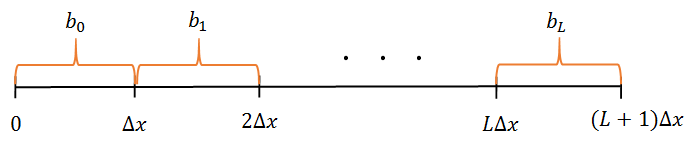
\includegraphics[width=14cm]{siatka_przestrzenna}
 \caption{Siatka przestrzenna}
 \label{fig:siatka_przestrzenna}
\end{figure}


\chapter{Makroskopowy model ruchu}
\section{Klasyfikacja modeli ruchu drogowego}
Modele ruchu drogowego mają na celu ukazanie rzeczywistego przepływu pojazdów w sposób czysto matematyczny. Ważnym kryterium doboru modelu jest przystępność jego implementacji informatycznej. Powszechnie klasyfikuje się 3 podejścia modelowe dla omawianego problemu \cite{CompareModels} - makroskopowy, mezoskopowy oraz mikroskopowy. Czasem \cite{multilevel} wyróżnia się także czwarte podejście - submikroskopowe. Jest to podział ze względu na poziom modelu. Najniższy poziom i najbardziej dokładny model gwarantuje podejście mikroskopowe. Rozważa ono pojazdy indywidualnie w czasoprzestrzeni. Przyspieszenie pojazdu jest wyliczane na podstawie dynamiki(prędkości, przyspieszenia) i pozycji pojazdu bezpośrednio przed nim. Model mezoskopowy zapewnia indywidualne rozróżnienie pojazdów, jednak ich zachowanie jest wyliczane na danych zagregowanych \cite{mesoscopic}. Przykładowo pojazdy są zgrupowane w grupę podróżującą z pewnego punktu startowego do celu. Inne modele \cite{mesoscopic2} mezoskopowe wyliczają dynamikę ruchu na podstawie aktualnego zatłoczenia drogi. Poziom mezoskopowy jest obliczeniowo bardziej opłacalny od mikroskopowego.
Wiele symulatorów stosujących model mezoskopowy oferuje symulację w czasie rzeczywistym dla sieci dróg całego miasta\cite{vu2017high}. Ideą modelu makroskopowego jest traktowanie ruchu ulicznego identycznie jak ruchu cieczy lub gazów. Po raz pierwszy w roku 1956 M. J. Lighthill i G. B. Whitham \cite{lwr} przedstawili pomysł przyrównania ruchu ulicznego na zatłoczonych drogach do przepływu wody w rzekach. Z tego powodu nie rozróżniamy w nim indywidualnie pojazdów, ani też nawet grupowo. Rozważamy natomiast gęstość ruchu w danym punkcie na drodze i czasie - czyli ilość pojazdów na danym odcinku drogi. Sposób w jaki poruszają się pojazdy jest wyliczany jedynie na podstawie gęstości ruchu. Jest to najmniej kosztowny obliczeniowo model. Właśnie w modelu makroskopowym zostało stworzone środowisko symulacyjne. Szczegóły modelu są przedstawione w następnym podrozdziale.

\section{Wstęp}
Istotą makroskopowego modelu ruchu jest pojęcie gęstości ruchu. Jest to zmienna stanowa określona dla każdego punktu drogi w czasie. Formalnie gęstość można rozumieć jako czynnik definiujący dynamikę ruchu. Im większa gęstość tym mniejsza prędkość ruchu. W niektórych artykułach gęstość ruchu \cite{helbing2001master} jest przedstawiona jako iloraz ilości pojazdów znajdujących się na pewnym odcinku i długości tego odcinka drogi. Nie są to jednak czysto matematyczne formalne definicje. W makroskopowym modelu nie rozróżniamy pojedynczych pojazdów, ani nawet grup, więc taka definicja gęstości ruchu może być odebrana jako nieścisła z ideą modelu. 
\section{Rozwój gęstości ruchu na drodze}
Makroskopowy model ruchu jest oparty o równanie różniczkowe (\ref{eq:main_diff_eq}) wraz z warunkiem początkowym (\ref{eq:p_init_eq}). Model makroskopowy traktuje ruch uliczny na drogach podobnie do przepływu wody w rzece[ref]. Gęstość ruchu można utożsamiać z polem powierzchni przekroju poprzecznego rzeki, co dla ustalonej szerokości rzeki - upraszcza się do wysokości wody w rzece. Istotną uwagą w tym miejscu jest zaznaczenie, iż rzeka zazwyczaj posiada pewien spadek, który zapewnia ruch cieczy ze źródła do ujścia. Ruch makroskopowy zdefiniowany przez równanie (\ref{eq:main_diff_eq}) z kolei odnosi się do rzeki która jest na całym swoim odcinku pozioma. W takim przypadku de facto nie ma zdefiniowanego zwrotu ruchu. \\Dla ustalonej drogi $e$ zmianę gęstości ruchu definiuje następujący układ równań:\\
\begin{numcases}{}
   p(x,0)=p_{0}(x) \label{eq:p_init_eq}
   \\
   \frac{\partial p(x,t)}{\partial t}+\frac{\partial f(p(x,t))}{\partial x}=0 \label{eq:main_diff_eq}
\end{numcases}
Gdzie $p(x,t)$ to gęstość ruchu w punkcie $x$ i czasie $t$. Wartość funkcji gęstości należy do przedziału $[0,p^{max}]$.\\
Równanie (\ref{eq:p_init_eq}) zakłada istnienie pewnej z góry nałożonej początkowej gęstości drogi $p_0(x)$.
Równianie (\ref{eq:main_diff_eq}) określa
wedle założeń modelu makroskopowego \cite{lwr} rozwój gęstości ruchu na drodze. Funkcja płynności ruchu $f$ powinna być wklęsła [ref]. W przedstawionym w tej pracy modelu funkcja ma następującą definicję:
\begin{numcases}{f(p)=}
   \lambda p & \text{dla } $p\in[0,p^{*}]$\\
   \lambda \cdot (2p^{*}-p) & \text{dla } $p\in(p^{*},p^{max}]$ 
\end{numcases}
Gdzie $\lambda$ jest stałym parametrem funkcji trójkątnej oraz $p^*=\frac{1}{2}p^{max}$.

\section{Dyskretyzacja makroskopowego modelu ruchu}
Niech będzie ustalona droga $e$ oraz jej siatka przestrzenna $b_l$. Celem jest przedstawienie wartości gęstości dla odcinków siatki przestrzennej w chwilach $k=0,1,...,K$.
Gęstość w odcinku $b_l$ i czasie $k$ jest zdefiniowana jako:
\[p_{l}^{k}=\int\limits_{{b_{l}}}{\frac{p(x,k)}{\Delta x}dx}. \addtag\]
Na podstawie (\ref{eq:main_diff_eq}) można wywnioskować, że:
\[\int\limits_{b_{l}} {p(x,k+1)- p(x,k)dx} +\int\limits_{k}^{k+1} f(b_{l+1},k)-f(b_{l},k))dk=0 \addtag \label{eq:calki-LWR} \]
Upraszczając otrzymujemy:
\[\Delta x(p_l^{k+1}-p_l^{k}) +\int\limits_{k}^{k+1} f(b_{l+1},k)-f(b_{l},k))dk=0=0 \addtag \]
Wartości gęstości zmieniają się w tylko w chwilach $k$. Wtedy wartości $f(b_{l+1},k)$ i $f(b_l,k)$ są stałe na całym przedziale całkowania $[k,k+1)$. Otrzymujemy równanie:
\[\Delta x(p_l^{k+1}-p_l^{k})  + (f(b_{l+1},k)-f(b_l,k))=0 \addtag \]
Rezultatem jest końcowy rekurencyjny wzór na gęstość ruchu:
\[p_l^{k+1}=p_l^{k}  -\frac{1}{\Delta x}  (f(b_{l+1},k)-f(b_l,k)) \addtag \]


\chapter{Model sieci dróg}
\section{Wstęp}
Ze względu na dużą złożoność końcowego modelu zostanie przedstawiony najpierw bardzo prosty, podstawowy model. W każdej kolejnej sekcji dodawane będą zmiany przybliżające do ostatecznej postaci. Jest to podejście pozwalające na proste przedstawienie modelu, który zawiera bardzo wiele aspektów m.in:
ujęcie sygnalizacji świetlnej, brak kolizyjnych manewrów, makroskopowy przepływ ruchu, przepływ ruchu na skrzyżowaniu, struktura sieci dróg. Zestawienie w jednej sekcji wszystkich tych kwestii byłoby bardzo przytłaczające.

\section{Wektor stanu drogi} \label{sec:wektor_stanu_drogi}
Wektor stanu jest strukturą w pełni przedstawiającą aktualny stan drogi. Dla każdego odcinka drogi składuje on wartości zmiennych stanuch. Początkowo zmienna stanowa jest identyfikowana jako ilość pojazdów na danym odcinku drogi. 
\subsection{Przykład} \label{subsec:example-single-road}
Niech będzie dana droga $e$ z wydzielonymi czterema odcinkami ${b_1,b_2,b_3,b_4}$. Przykładowy wektor stanu to
\[\textbf{x(t)}=\begin{bmatrix}
2 \\ 4 \\ 3 \\ 0
\end{bmatrix} \addtag \]
Zawiera on w sobie następujące informacje dla chwili t:
\begin{itemize}
	\item Są 2 pojazdy na odcinku $b_1$
	\item Są 4 pojazdy na odcinku $b_2$
	\item Są 3 pojazdy na odcinku $b_3$
	\item Nie ma żadnego pojazdu na odcinku $b_4$
\end{itemize}

\begin{figure}[H]
	\centering
	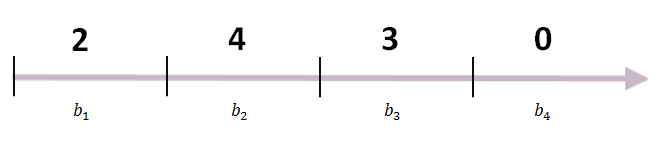
\includegraphics[width=14cm]{single_road_example}
	\caption{Droga z ilością pojazdów na poszczególnych odcinkach}
	\label{fig:single_road}
\end{figure}
\section{Rozwój wektora stanu jednej drogi}
Początkowy model przepływu pojazdów zakłada, iż wszystkie pojazdy w chwili t+1 są o jeden odcinek dalej w swojej podróży niż w momencie $t$. Założone jest, iż żadne nowe pojazdy nie pojawiają się w sieci dróg, a pojazdy będące w chwili $t$ w ostatnim odcinku drogi układ. Formalnym wzorem definiującym rozwój wektora stanu jest:
\[\textbf{x(t+1)}=\textbf{Ax(t)} \addtag \label{eq:single_road} \]
Gdzie $A$ jest macierzą systemu. Definiuje ona sposób przepływu pojazdów. $A$ jest rzadką, kwadratową macierzą o wartościach równych 1 jedynie bezpośrednio 1 wiersz pod główną przekątną macierzy. Takie wartości gwarantują przepływ pojazdów o jeden odcinek w jednym interwale czasowym.
\subsection{Przykład}
Dla przykładu przedstawionego w (\ref{subsec:example-single-road}) zostanie przedstawiony rozwój wektora stanu. Niech zatem
\def \xZero {\begin{bmatrix}
	2 \\ 4 \\ 3 \\ 0
	\end{bmatrix}}
\[\textbf{x(0)}=\xZero \addtag \]
Macierzą systemu jest:
\def \A {\begin{bmatrix}
		0 & 0 & 0 & 0 \\
		1 & 0 & 0 & 0 \\
		0 & 1 & 0 & 0 \\
		0 & 0 & 1 & 0 \\
\end{bmatrix}}

\[
\textbf{A}=\A \addtag
\]
Wedle wzoru (\ref{eq:single_road}) wyliczone zostają kolejne wartości wektora stanu.
\def \xI {\begin{bmatrix}
		0 \\ 2 \\ 4 \\ 3
\end{bmatrix}}
\[
\textbf{x(1)}=\textbf{Ax(0)}=\A \xZero = \xI \addtag
\]
\def \xII {\begin{bmatrix}
		0 \\ 0 \\ 2 \\ 4
\end{bmatrix}}
\[
\textbf{x(2)}=\textbf{Ax(1)}=\A \xI = \xII \addtag
\]
\def \xIII {\begin{bmatrix}
		0 \\ 0 \\ 0 \\ 2
\end{bmatrix}}
\[
\textbf{x(3)}=\textbf{Ax(2)}=\A \xII = \xIII \addtag
\]
\def \xIV {\begin{bmatrix}
		0 \\ 0 \\ 0 \\ 0
\end{bmatrix}}
\[
\textbf{x(4)}=\textbf{Ax(3)}=\A \xIII = \xIV \addtag
\]

\section {Wektor stanu sieci dróg}
W rozdziale (\ref{sec:wektor_stanu_drogi}) przedstawiony został wektor stanu dla pojedynczej drogi. W tym rozdziale zostanie sformułowany wektor stanu dla bardziej ogólnego przypadku - sieci dróg. Sposób przedstawienia wartości stanuch jednak jest bardzo podobny. Każda z dróg $e_1,...,e_n$ ma $k$ wydzielonych odcinków oznaczanych jako $b_1,...,b_{nk}$. Dla każdego z odcinków definiowana jest wartość stanowa.

\subsection{Przykład} \label{subsec:wektor_stanu_siec_przyklad}
Niech będzie dana sieć składająca się z trzech dróg $E=\{e_1,e_2,e_3\}$. Dla każdej drogi zostaną wydzielone 2 odcinki. Przykładowy wektor stanu
\def \xzero {\begin{bmatrix}
		8 \\ 4 \\ 3 \\ 0 \\ 1 \\ 5
\end{bmatrix}}

\[\textbf{x(t)}=\xzero \addtag \]
Zawiera w sobie następujące informacje dotyczące ilości pojazdów na poszczególnych odcinkach w chwili t:
\begin{itemize}
	\item $\boldsymbol{b_1}$ - Na pierwszym odcinku drogi $e_1$ jest 8 pojazdów
	\item $\boldsymbol{b_2}$ - Na drugim odcinku drogi $e_1$ są 4 pojazdy 
	\item $\boldsymbol{b_3}$ - Na pierwszym odcinku drogi $e_2$ są 3 pojazdy 
	\item $\boldsymbol{b_4}$ - Na drugim odcinku drogi $e_2$ nie ma żadnych pojazdów 
	\item $\boldsymbol{b_5}$ - Na pierwszym odcinku drogi $e_3$ jest 1 pojazd
	\item $\boldsymbol{b_6}$ -Na drugim odcinku drogi $e_3$ jest 5 pojazdów
\end{itemize}

\begin{figure}[H]
	\centering
	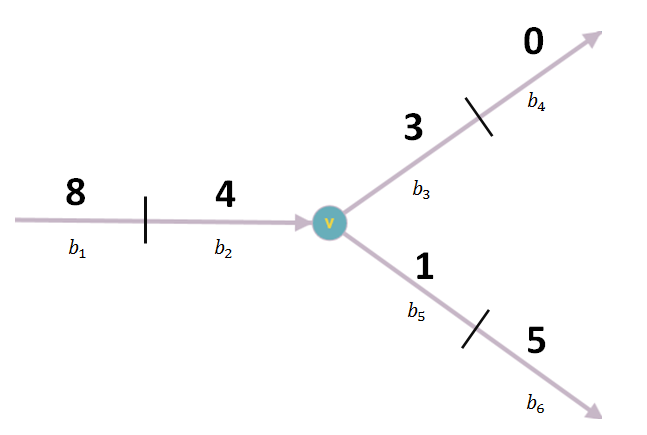
\includegraphics[width=14cm]{3_single_road}
	\caption{Sieć dróg z ilościami pojazdów na poszczególnych odcinkach}
	\label{fig:3_single_road}
\end{figure}

\section{Rozwój wektora stanu sieci dróg}
Przepływ pojazdów niezmiennie jest oparty o założenie, iż w trakcie trwania jednego interwału czasowego pojazdy pokonują 1 odcinek drogi. Równaniem systemu pozostaje $\textbf{x(t+1)=Ax(t)}$, gdyż do układu niezmiennie nie wpływają nowe pojazdy.\\ \\
Macierz systemu $\textbf{A}$ powinna uwzględnić przepływy pojazdów na skrzyżowaniach. W tym momencie należy przedstawić następującą definicję macierzy $\textbf{A}$:\\
Wartości macierzy \textbf{A} określają jaka część pojazdów z odcinka zadanego przez indeks kolumny przejeżdża do odcinka zadanego przez indeks wiersza.


\subsection{Przykład}
Dla przykładu (\ref{subsec:wektor_stanu_siec_przyklad}) przedstawiony zostanie rozwój wektora stanu. Założone zostaje, iż $75 \%$ pojazdów będących na odcinku $b_2$ opuszcza skrzyżowanie na odcinku $b_3$ a pozostałe $25 \%$ przejeżdża do $b_5$.

\begin{figure}[H]
	\centering
	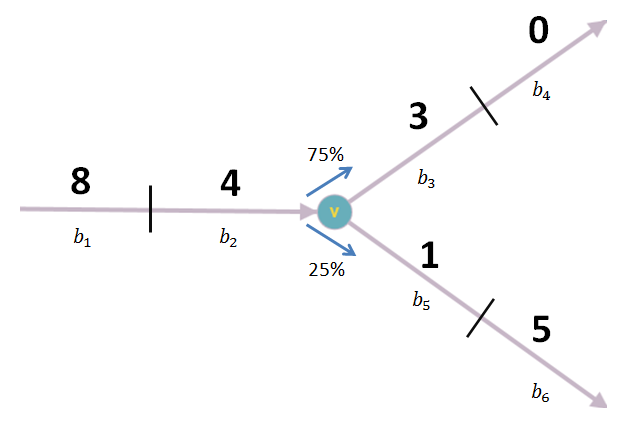
\includegraphics[width=14cm]{3_single_road_lights}
	\caption{}
	\label{fig:3_single_road}
\end{figure}

Wtedy:
\def \A{
\begin{bmatrix}
	0 & 0    & 0 & 0 & 0 & 0 \\
	1 & 0    & 0 & 0 & 0 & 0 \\
	0 & 75\% & 0 & 0 & 0 & 0 \\
	0 & 0    & 1 & 0 & 0 & 0 \\
	0 & 25\% & 0 & 0 & 0 & 0 \\
	0 & 0    & 0 & 0 & 1 & 0 
\end{bmatrix}
}
\begin{equation*}
\textbf{A}=
\begin{blockarray}{*{6}{c} l}
\begin{block}{*{6}{>{$\footnotesize}c<{$}} l}
$b_1$ & $b_2$ & $b_3$ & $b_4$ & $b_5$ & $b_6$ \\
\end{block}
\begin{block}{[*{6}{c}]>{$\footnotesize}l<{$}}
0 & 0 & 0 & 0 & 0 & 0 & $b_1$ \\
1 & 0 & 0 & 0 & 0 & 0 & $b_2$ \\
0 & 75\% & 0 & 0 & 0 & 0 & $b_3$ \\
0 & 0 & 1 & 0 & 0 & 0 & $b_4$ \\
0 & 25\% & 0 & 0 & 0 & 0 & $b_5$ \\
0 & 0 & 0 & 0 & 1 & 0 & $b_6$ \\
\end{block}
\end{blockarray} \addtag
\end{equation*}
Niech zatem zgodnie z rysunkiem \ref{fig:3_single_road}:
\[\textbf{x(0)}=\xzero \]
Kolejne wartości wektora stanu to:
\def \xI{\begin{bmatrix}
	0 \\ 8 \\ 3 \\ 3 \\ 1 \\ 1
\end{bmatrix}}
\def \xII{\begin{bmatrix}
		0 \\ 0 \\ 6 \\ 3 \\ 2 \\ 1
	\end{bmatrix}}
\def \xIII{\begin{bmatrix}
		0 \\ 0 \\ 0 \\ 6 \\ 0 \\ 2
\end{bmatrix}}
\[
\textbf{x(1)}=\textbf{Ax(0)}=\A \xzero = \xI
\]
\[
\textbf{x(2)}=\textbf{Ax(1)}=\A \xI = \xII
\]
\[
\textbf{x(3)}=\textbf{Ax(2)}=\A \xII = \xIII
\]

\newpage
\section{Wprowadzenie sygnalizacji świetlnej}
Kolejnym etapem rozwoju modelu jest wprowadzenie sygnalizacji świetlnej. Warto zauważyć, że do tej pory rozważane układy były pozbawione jakiegokolwiek sterowania, czego bezpośrednim skutkiem była niezmienność macierzy $\textbf{A}$ w czasie. W chwili pojawienia się sygnalizacji świetlnej macierz systemu będzie oparta o aktualną fazę sygnalizacji świetlnej. Równanie systemu pozostaje takie samo jak w przypadku braku sygnalizacji świetlnej z jedną małą różnicą:
\[\textbf{x(t+1)}=\textbf{A(t)x(t)} \addtag \]
Macierz systemu jest zmienna w czasie, zatem w miejse $\textbf{A}$ pojawiło się $\textbf{A(t)}$. \\ \\
Dla rozważanej sieci dróg zostaje przedstawiona \textbf{macierz topologii} układu $\textbf{T}$. Jej wartości podobnie jak macierzy $\textbf{A}$ odnoszą się do tego jaka część pojazdów z odcinka zadanego przez indeks kolumny przejeżdża do odcinka zadanego przez indeks wiersza. Macierz $\textbf{A}$ dotyczy jednak możliwych przejazdów w konkretnej fazie sygnalizacji świetlnej. Natomiast macierz topologii $\textbf{T}$ odnosi się do wszystkich możliwych przejazdów -  uwzględniając wszystkie fazy sygnalizacji świetlnej i jest stała w czasie. \\ \\
\noindent
\textbf{Macierz sterowania} (sygnalizacją świetlną) oznaczana będzie jako $\textbf{S(t)}$. Ustala ona macierz systemu na podstawie następującej równości:
\[\textbf{A(t)}=\textbf{S(t)T} \addtag \]
Jeśli $S(t)$ określa przejazdy, które są rzeczywiście możliwe w układzie, to:
\[\textbf{A(t)}=\textbf{S(t)} \addtag \]
Zatem celem wprowadzenia macierzy topologii oprócz przedstawienia wszystkich możliwych przejazdów jest także walidacja przejazdów zadanych przez macierz sterowania $\textbf{S(t)}$.

\subsection{Przykład}
Rozważony zostanie przykład sieci trzech dróg $e_1,e_2,e_3$. Każda z nich jest podzielona na dwa odcinki. Drogi $e_1$ i $e_2$ zbiegają się na skrzyżowaniu z sygnalizacją świetlną. Założone jest, że sygnalizacja zmienia się w każdym kroku czasowym, jednak w międzyczasie przez jeden interwał czasowy jest żółte światło dla obydwu dróg. Matematycznie ujmując żółte światło jest równoważne czerwonemu - pojazdy czekają na skrzyżowaniu. Początkowy stan sieci przedstawia rysunek:
\begin{figure}[H]
	\centering
	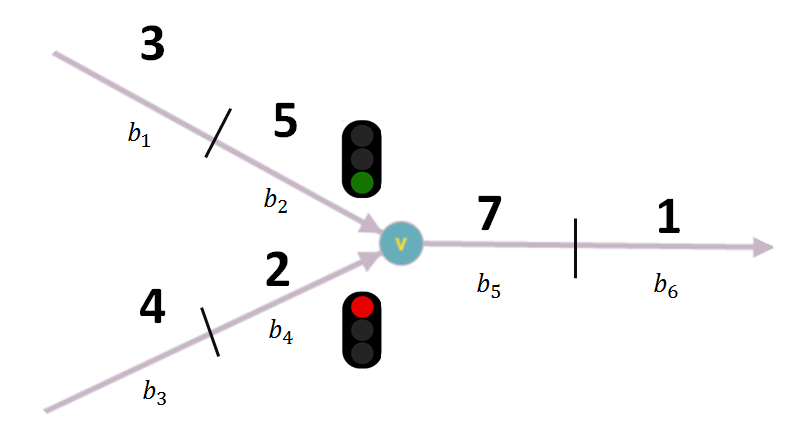
\includegraphics[width=14cm]{3_drogi_sygnalizacja}
	\caption{Sieć dróg z sygnalizacją świetlną w chwili t=0}
	\label{fig:3_drogi_sygnalizacja}
\end{figure}

Należy zastanowić się nad macierzą topologii układu $\textbf{T}$. Jest ona następująca:
\begin{equation*}
\textbf{T}=
\begin{blockarray}{*{6}{c} l}
\begin{block}{*{6}{>{$\footnotesize}c<{$}} l}
$b_1$ & $b_2$ & $b_3$ & $b_4$ & $b_5$ & $b_6$ \\
\end{block}
\begin{block}{[*{6}{c}]>{$\footnotesize}l<{$}}
0 & 0 & 0 & 0 & 0 & 0 & $b_1$ \\
1 & \colorbox{red!30}{1} & 0 & 0 & 0 & 0 & $b_2$ \\
0 & 0 & 0 & 0 & 0 & 0 & $b_3$ \\
0 & 0 & 1 & \colorbox{red!30}{1} & 0 & 0 & $b_4$ \\
0 & \colorbox{green!30}{1} & 0 & \colorbox{green!30}{1} & 0 & 0 & $b_5$ \\
0 & 0 & 0 & 0 & 1 & 0 & $b_6$ \\
\end{block}
\end{blockarray} \addtag
\end{equation*}
\begin{itemize}
	\item Wartości w kolumnach $b_1,b_3,b_5$ są równe 1 tylko w wierszach odpowiadającym odcinkom $b_2,b_4,b_6$, co wynika z tego, że pojazdy będące na odcinkach $b_1,b_3,b_5$ mają tylko możliwość przejazdu do odpowiednio $b_2,b_4,b_6$.
	\item Wartości w kolumnie $b_6$ są zerowe, gdyż pojazdy z odcinku $b_6$ opuszczają układ.
	\item Najbardziej interesujące są kolumny $b_2$ i $b_4$. Odpowiadają one odcinkom leżącym bezpośrednio przed skrzyżowaniem. Obydwie kolumny posiadają dwie wartości 1, gdyż pojazdy będące na odcinkach $b_2,b_4$ mają dwie możliwości przejazdu. Pojazdy będące na odcinku $b_2$ mogą przejechać przez skrzyżowanie i wjechać na $b_5$, albo pozostać dalej na $b_2$ w przypadku czerwonego światła. Analogiczna sytuacja dotyczy pojazdów na odcinku $b_4$. \colorbox{green!30}{Zielone} i \colorbox{red!30}{czerwone} tło określają przy jakiej sygnalizacji świetlnej opisany przejazd jest możliwy.
\end{itemize}

\def \xzero{
	\begin{bmatrix}
		4 \\ 5 \\ 4 \\ 2 \\ 7 \\ 1
	\end{bmatrix}
}
Początkowy wektor stanu (zgodny z rysunkiem \ref{fig:3_drogi_sygnalizacja}) to:
\[\textbf{x(0)}= \xzero \]
Macierz stanu w momentach $t=0,4$ uwzględnia zielone światło dla drogi $e_1$ oraz czerwone dla $e_2$.
\def \aeI{
\begin{bmatrix}
	0 & 0                     & 0 & 0 & 0 & 0 \\
	1 & \colorbox{red!30}{0}  & 0 & 0 & 0 & 0 \\
	0 & 0                     & 0 & 0 & 0 & 0 \\
	0 & 0                     & 1 & \colorbox{red!30}{1} & 0 & 0 & \\
	0 & \colorbox{green!30}{1}  & 0 & \colorbox{green!30}{0} & 0 & 0 \\
	0 & 0                     & 0 & 0 & 1 & 0 \\
\end{bmatrix}

}

\begin{equation*}
\boldsymbol{A_{e_1}}=
\begin{blockarray}{*{6}{c} l}
\begin{block}{*{6}{>{$\footnotesize}c<{$}} l}
$b_1$ & \colorbox{green!30}{$b_2$} & $b_3$ & \colorbox{red!30}{$b_4$} & $b_5$ & $b_6$ \\
\end{block}
\begin{block}{[*{6}{c}]>{$\footnotesize}l<{$}}
0 & 0                     & 0 & 0 & 0 & 0 & $b_1$ \\
1 & \colorbox{red!30}{0}  & 0 & 0 & 0 & 0 & $b_2$ \\
0 & 0                     & 0 & 0 & 0 & 0 &  $b_3$ \\
0 & 0                     & 1 & \colorbox{red!30}{1} & 0 & 0 & $b_4$ \\
0 & \colorbox{green!30}{1}  & 0 & \colorbox{green!30}{0} & 0 & 0 & $b_5$ \\
0 & 0                     & 0 & 0 & 1 & 0 & $b_6$ \\
\end{block}
\end{blockarray} \addtag
\end{equation*}
Macierz stanu w momentach $t=1,3,5$ uwzględnia żółte światło zarówno dla $e_1$ jak i $e_2$. Jak zostało już wspomniane, jest ono równoważne czerwonemu światłu.
\begin{equation*}
\boldsymbol{A_{yellow}}=
\begin{blockarray}{*{6}{c} l}
\begin{block}{*{6}{>{$\footnotesize}c<{$}} l}
$b_1$ & \colorbox{red!30}{$b_2$} & $b_3$ & \colorbox{red!30}{$b_4$} & $b_5$ & $b_6$ \\
\end{block}
\begin{block}{[*{6}{c}]>{$\footnotesize}l<{$}}
0 & 0                     & 0 & 0 & 0 & 0 & $b_1$ \\
1 & \colorbox{red!30}{1}  & 0 & 0 & 0 & 0 & $b_2$ \\
0 & 0                     & 0 & 0 & 0 & 0 &  $b_3$ \\
0 & 0                     & 1 & \colorbox{red!30}{1} & 0 & 0 & $b_4$ \\
0 & \colorbox{green!30}{0}  & 0 & \colorbox{green!30}{0} & 0 & 0 & $b_5$ \\
0 & 0                     & 0 & 0 & 1 & 0 & $b_6$ \\
\end{block}
\end{blockarray} \addtag
\end{equation*} 
Macierz stanu w momencie $t=2$ uwzględnia zielone światło dla drogi $e_2$ oraz czerwone dla $e_1$.
\begin{equation*}
\boldsymbol{A_{e_2}}=
\begin{blockarray}{*{6}{c} l}
\begin{block}{*{6}{>{$\footnotesize}c<{$}} l}
$b_1$ & \colorbox{red!30}{$b_2$} & $b_3$ & \colorbox{green!30}{$b_4$} & $b_5$ & $b_6$ \\
\end{block}
\begin{block}{[*{6}{c}]>{$\footnotesize}l<{$}}
0 & 0                     & 0 & 0 & 0 & 0 & $b_1$ \\
1 & \colorbox{red!30}{1}  & 0 & 0 & 0 & 0 & $b_2$ \\
0 & 0                     & 0 & 0 & 0 & 0 &  $b_3$ \\
0 & 0                     & 1 & \colorbox{red!30}{0} & 0 & 0 & $b_4$ \\
0 & \colorbox{green!30}{0}  & 0 & \colorbox{green!30}{1} & 0 & 0 & $b_5$ \\
0 & 0                     & 0 & 0 & 1 & 0 & $b_6$ \\
\end{block}
\end{blockarray} \addtag
\end{equation*}






\def \xzero{
	\begin{bmatrix}
		4 \\ 5 \\ 4 \\ 2 \\ 7 \\ 1
	\end{bmatrix}
}

\def \xzero{
	\begin{bmatrix} 3 \\ 5 \\ 4 \\ 2 \\ 7 \\ 1 \end{bmatrix}
}
\def \xI{
	\begin{bmatrix} 0 \\ 3 \\ 0 \\ 6 \\ 5 \\ 7 \end{bmatrix}
}
\def \xII{
	\begin{bmatrix} 0 \\ 3 \\ 0 \\ 6 \\ 0 \\ 5 \end{bmatrix}
}
\def \xIII{
	\begin{bmatrix} 0 \\ 3 \\ 0 \\ 0 \\ 6 \\ 0 \end{bmatrix}
}
\def \xIV{
	\begin{bmatrix} 0 \\ 3 \\ 0 \\ 0 \\ 0 \\ 6 \end{bmatrix}
}
\def \xV{
	\begin{bmatrix} 0 \\ 0 \\ 0 \\ 0 \\ 3 \\ 0 \end{bmatrix}
}
\def \aeI{
	\begin{bmatrix}
		0 & 0                     & 0 & 0 & 0 & 0 \\
		1 & \colorbox{red!30}{0}  & 0 & 0 & 0 & 0 \\
		0 & 0                     & 0 & 0 & 0 & 0 \\
		0 & 0                     & 1 & \colorbox{red!30}{1} & 0 & 0 & \\
		0 & \colorbox{green!30}{1}  & 0 & \colorbox{green!30}{0} & 0 & 0 \\
		0 & 0                     & 0 & 0 & 1 & 0 \\
	\end{bmatrix}	
}
\def \aeII{
	\begin{bmatrix}
		0 & 0                     & 0 & 0 & 0 & 0 \\
		1 & \colorbox{red!30}{1}  & 0 & 0 & 0 & 0 \\
		0 & 0                     & 0 & 0 & 0 & 0 \\
		0 & 0                     & 1 & \colorbox{red!30}{0} & 0 & 0 & \\
		0 & \colorbox{green!30}{0}  & 0 & \colorbox{green!30}{1} & 0 & 0 \\
		0 & 0                     & 0 & 0 & 1 & 0 \\
	\end{bmatrix}	
}
\def \ayellow{
	\begin{bmatrix}
		0 & 0                     & 0 & 0 & 0 & 0 \\
		1 & \colorbox{red!30}{1}  & 0 & 0 & 0 & 0 \\
		0 & 0                     & 0 & 0 & 0 & 0 \\
		0 & 0                     & 1 & \colorbox{red!30}{1} & 0 & 0 & \\
		0 & \colorbox{green!30}{0}  & 0 & \colorbox{green!30}{0} & 0 & 0 \\
		0 & 0                     & 0 & 0 & 1 & 0 \\
	\end{bmatrix}
	
}

	
	\begin{tabular}{| c | c | c | Sc |}
		\hline
		t & $\textbf{x(t)}$ & $\textbf{A(t)}$ & Rysunek stanu układu \\
		\hline
		0 & $\xzero$  & $\aeI$ & \cincludegraphics[height=3cm]{3_drogi_sygnalizacja_0} \\
		\hline 
		1 & $\xI$  & $\ayellow$ & \cincludegraphics[height=3cm]{3_drogi_sygnalizacja_1} \\
		\hline
		2 & $\xII$  & $\aeII$ & \cincludegraphics[height=3cm]{3_drogi_sygnalizacja_2} \\
		\hline
		3 & $\xIII$  & $\ayellow$ & \cincludegraphics[height=3cm]{3_drogi_sygnalizacja_3} \\
		\hline
		4 & $\xIV$  & $\aeI$ & \cincludegraphics[height=3cm]{3_drogi_sygnalizacja_4} \\
		\hline
		5 & $\xV$  & $\ayellow$ & \cincludegraphics[height=3cm]{3_drogi_sygnalizacja_5} \\
		\hline
	\end{tabular}

\section{Wprowadzenie źródeł ruchu }
Wszystkie poprzednie przykłady układów ruchu drogowego szybko kończyły się stanem w którym nie było już żadnych pojazdów na drogach. W tym rozdziale zostanie przedstawiony sposób napływania nowych pojazdów do układu. Drogi układu, które nie rozpoczynają się na skrzyżowaniu będą nazywane drogami zródłowymi. Niech zbiór wszystkich dróg zródłowych to $E_s={e_1,...,e_k}$. Wektorem zródła w chwili $t$ nazywany bedzie wektor:
\[\boldsymbol{u(t)}=\begin{bmatrix} u_1 \\ ... \\ u_k \end{bmatrix} \]
Równanie systemu uwzględniające zródła ruchu to:
\[\textbf{x(t+1)}=\textbf{A(t)x(t)} + \textbf{Bu(t)} \label{eq:stan_u}   \addtag{}\]
Gdzie $B$ jest macierzą odpowiedzialną za zrzutowanie pojazdów napływających do dróg zródłowych do odpowiednich odcinków.

\subsection{Przykład dla pojedynczej drogi}
Niech dana będzie droga $e$ podzielona na 4 odcinki $b_1,b_2,b_3,b_4$. Początkowo niech wektor stanu to
\[\textbf{x(0)}=\begin{bmatrix} 2 \\ 4 \\ 3 \\ 0 \end{bmatrix} \]
Dane są następujące wektory zrodlowe:
\[\textbf{u(0)}=[7] \;\;\; \textbf{u(1)}=[3] \;\;\; \textbf{u(2)}=[5]\]
Są to wektory o wymiarze 1, gdyż w układzie jest tylko 1 droga.
Spodziewany następny wektor stanu to:\[\textbf{x(1)}=\begin{bmatrix} 7 \\ 2 \\ 4 \\ 3 \end{bmatrix} \addtag \] gdyż na pierwszym odcinku pojawia się 7 pojazdów ze zródła \textbf{u(0)}, a pozostałe pojazdy przejeżdżają jeden odcinek drogi. Oczywiście $\textbf{Ax(0)}=\begin{bmatrix} 0 & 2 & 4 & 3 \end{bmatrix}^T$, zatem koniecznie
$\textbf{Bu(0)}= \begin{bmatrix} 7 & 0 & 0 & 0 \end{bmatrix}^T$
Macierz $\boldsymbol{B}$ zatem musi być dla tego układu następująca:
\[\boldsymbol{B}=\begin{bmatrix}
1 \\ 0 \\ 0 \\ 0 \addtag
\end{bmatrix}\]
Jest ona stała w czasie. Wartości kolejnych wektorów stanu wyznaczone ze wzoru (\ref{eq:stan_u}) to:
\[\textbf{x(2)}=\begin{bmatrix}
3 \\ 7 \\ 2 \\ 4 
\end{bmatrix}\]
\[\textbf{x(3)}=\begin{bmatrix}
5 \\ 3 \\ 7 \\ 2 
\end{bmatrix}\]
\subsection{Przykład dla złożonej sieci dróg}
Niech dany będzie układ składający się z 5 dróg, z czego każda jest podzielona na dwa odcinki. Strukturę sieci dróg przedstawia poniższy rysunek.
\begin{figure}[H]
	\centering
	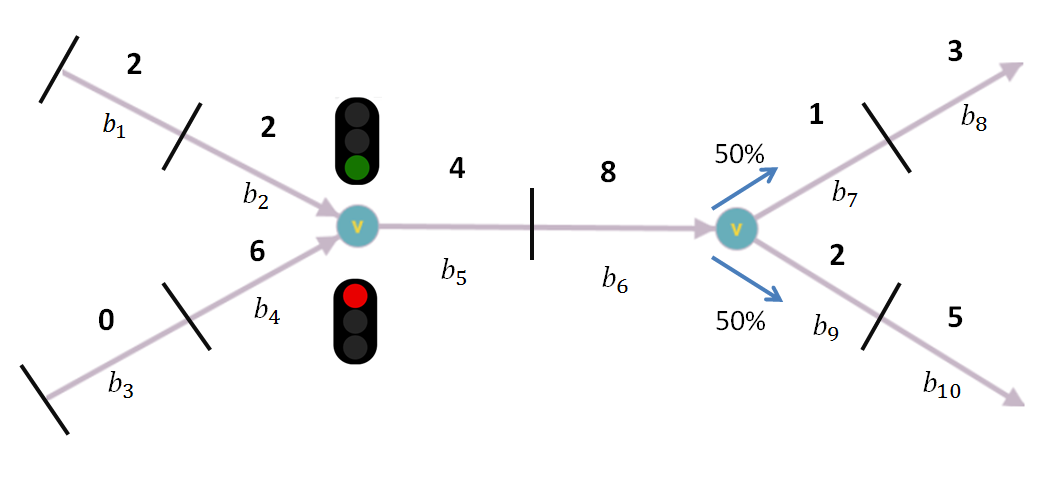
\includegraphics[width=14cm]{5_drog}
	\caption{Złożona sieć dróg}
	\label{fig:5_drog}
\end{figure}
Dalszy rozwój ruchu-
Do zrobienia :)
\section{Wprowadzenie gęstości ruchu}
Do zrobienia :)
\section{Układy symulacyjne}
Do zrobienia :)

\chapter{Przedstawienie problemu optymalizacyjnego}

\bibliographystyle{IEEEtran}

\chapter{Przegląd metod optymalizacyjnych}
\section{Kategorie uczenia maszynowego}
Uczenie maszynowe to dziedzina wchodząca w skład nauk zajmujących się sztuczną inteligencją. Samo uczenie w najprostszym kształcie może być rozumiane jako dobór parametrów na podstawie dostępnych danych. Uczenie maszynowe jest powszechnie dzielone na 3 kategorie nauki \cite{machineLearningClassification}.
\begin{enumerate}
\item \textbf{Nadzorowane} \\
Dane używane do uczenia nazywane są zbiorem treningowym. Każdy pojedynczy element zbioru treningowego ma informacje wejściowe oraz pewną pożądaną wartość wyjściową. W trakcie uczenia algorytm dopasowuje swoje parametry tak aby na podstawie danych wejściowych mógł przewidzieć wartość wyjściową. Przykładami uczenia nadzorowanego jest np. rozpoznawanie tekstu pisanego, detekcja obiektów na zdjęciach.
\item \textbf{Nienadzorowane}
Uczenie nienadzorowane różni się od nadzorowanego tym, że nie  są znane pożądane wartości wyjściowe. Celem nauki jest na podstawie podobieństw poszczególnych elementów zgrupowanie ich do odpowiednich klas. Przykładem uczenia nienadzorowanego może być np. klasyfikacja gatunków drzew na podstawie wiedzy o ich wysokościach i szerokości korony drzew.
\item \textbf{Wzmocnione}
W środowisku uczenia ze wzmocnieniem istnieje agent, który jest odpowiedzialny za podejmowanie pewnych decyzji. Każda decyzja ma wpływ na stan środowiska, które zwraca agentowi nagrodę. Celem uczenia ze wzmocnieniem jest ustalenie strategii maksymalizującej skumulowaną wartość nagród.
\end{enumerate}
Ze wszystkich trzech kategorii uczenie ze wzmocnieniem odpowiada problemowi rozważanym w rozdziale Y. Szczegółowy opis uczenia ze wzmocnieniem zostanie przedstawiony w następnej sekcji.
\section{Uczenie ze wzmocnieniem}
Schemat uczenia ze wzmocnieniem składa się z następujących elementów:
\begin{enumerate}
\item \textbf{Agent} jest odpowiedzialny za podejmowanie pewnych decyzji. Ma on wiedzę na temat obecnego stanu środowiska i otrzymuje w każdym kroku czasowym sygnał nagrody. Jego decyzje wpływają na stan środowiska.
\item \textbf{Środowisko} jest przestrzenią posiadającą dynamiczny stan widoczny dla agenta. Chociaż to agent podejmuje akcje, to środowisko ma zdefiniowany model zmiany stanu. Model zmiany stanu może być stochastyczny oraz niewidoczny dla agenta. Oznacza to, że dwie te same akcje podjęte w tym samym stanie nie zawsze przyniosą identyczny następny stan. Innymi słowy agent nie może być stuprocentowo pewny rezultatów swoich akcji. Środowisko jest także nadawcą sygnału nagrody.
\item \textbf{Strategia} definiuje sposób doboru akcji przez agenta w danej chwili. Jest to funkcja, która przyjmuje stan środowiska i zwraca akcje, która ma być przeprowadzona. 
\item \textbf{Sygnał nagrody} definiuje cel problemu uczenia ze wzmocnieniem. W każdym kroku czasowym środowisko wysyła agentowi liczbę rzeczywistą, która jest nazywana nagrodą(reward). Wartości nagród są czynnikiem wpływającym na zmianę strategii, gdyż zadaniem agenta jest maksymalizacja nagród. Wartość nagród zatem definiuje, które zdarzenia są dobre, a które złe dla agenta. Biologicznym odpowiednikiem dodatniej nagrody jest przyjemność, a ujemnej - ból. 
\item \textbf{Funkcja wartości} zwraca wartość stanu czyli oczekiwaną sumę nagród jakie agent osiągnie w przyszłości będąc aktualnie w tym stanie. 
\end{enumerate}
\begin{figure}[H]
  \centering
    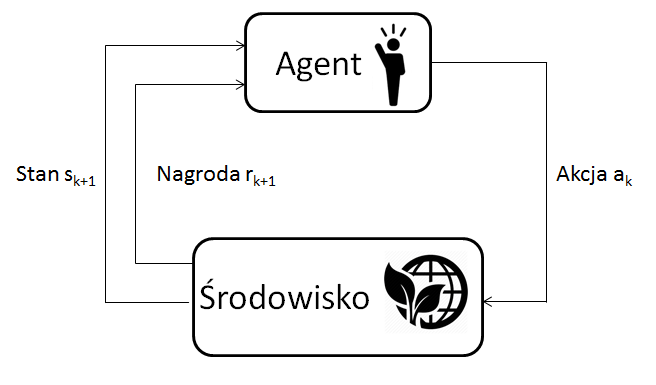
\includegraphics[width=14cm]{agent-srodowisko}
 \caption{Interakcje pomiędzy agentem a środowiskiem.}
 \label{fig:agent-srodowisko}
\end{figure}
\newpage
Algorytmy uczenia ze wzmocnieniem zazwyczaj stosuje się do rozwiązywania problemu procesu decyzyjnego Markowa. Sam \textbf{proces decyzyjny Markowa} jest zdefiniowany jako uporządkowana czwórka $(S,A,P_a,R_a)$, gdzie:
\begin{enumerate}
\item $S$ to zbiór stanów
\item $A$ to zbiór akcji. Notacją $A_s$ oznaczane są możliwe akcje dla stanu $s$.
\item $P_a(s,s')=Pr(s_{t+1}=s'|s_t=s,a_t=a)$ to prawdopodobieństwo, że akcja $a$ wykonana w stanie $s$ w chwili $t$ doprowadzi do stanu $s'$ w chwili $t+1$.
\item $R_a(s,s')$ to oczekiwana nagroda otrzymana w wyniku akcji podjętej w stanie $s$ prowadzącej do stanu $s'$.
\end{enumerate}

Problemem procesu decyzyjnego Markowa jest odnalezienie optymalnej strategii. Strategia określona jest jako funkcja $\pi(s)$ przyjmująca jako argument stan, a zwracająca podejmowaną akcję. Celem optymalizacji jest odnalezienie strategii maksymalizującej wartość:
\[
G=\sum_{k=0}^{K} \gamma^k R_{k} \addtag \label{eq:Markov_maximize}
\]
Chociaż strategii $\pi(s)$ nie ma we wzorcze \ref{eq:Markov_maximize}, to strategia wpływa na otrzymywane nagrody $R_{k}$ w każdej chwili $k$.\\
$\gamma \in (0,1]$ jest czynnikiem dyskontującym. Idea dyskontowania nagród zaczerpnięta jest z rachunku finansowego. Przykładowo wpływ 1000 złotych po upływie roku czasu jest z pewnością bardziej wartościowy niż za 20 lat. Innymi słowy - pieniądze są liczone w czasie i tak samo należy postępować z nagrodami. Im wartość $\gamma$ jest bliższa 0 tym bardziej istotne są początkowe nagrody. Dla $\gamma=1$ wszystkie nagrody są równie istotne - bez względu na czas ich otrzymania.\\
Analogicznie do (\ref{eq:Markov_maximize}) jest ustalona funkcja wartości stanu. Jako wartość stanu $s$ określone jest:
\[
G_t=\sum_{k=t}^{K} \gamma^k R_{k}=R_{t}+\gamma R_{t+1}+\gamma^{2} R_{t+2}+...+\gamma^{K}R_K \addtag \label{eq:Markov_state_value_G}
\]
Zostanie przedstawiony teraz przykład obliczeniowy. Agent podejmuje decyzje na których podstawie otrzymuje ciąg  nagród $R_0=0, R_1=2,R_2=6,R_3=-1,R_4=2,R_5=1$. Czynnik dyskontujący $\gamma$ jest równy 0,9. Jaka jest wartość $G$ oraz $G_1,G_2,G_3,G_4,G_5$?\\
\begin{figure}[H]
  \centering
    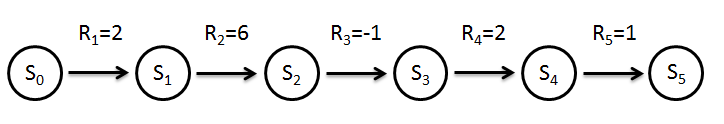
\includegraphics[width=14cm]{rewards-graph}
 \caption{Ciąg nagród i stanów.}
 \label{fig:agent-srodowisko}
\end{figure}\noindent
Najłatwiej obliczenia rozpocząć od $G_5$, ponieważ
\[G_{t}=R_{t}+\gamma G_{t+1} \label{eq:G_reccurential} \addtag \].\\
$G_5=R_5=1$.\\
$G_4=R_4+\gamma G_{5}=\;\;2+0,9\cdot 1=2,9$\\
$G_3=R_3+\gamma G_{4}=\!-1+0,9\cdot2.9=1,61$\\
$G_2=R_2+\gamma G_{3}=\;\;6+0,9\cdot1,61 \approx 7,45$\\
$G_1=R_1+\gamma G_{2}=\;\;2+0,9\cdot 7,45 \approx 8,70$\\
$G\;\,=R_0+\gamma G_{1}=\;\;0+0,9\cdot 8,70 \approx 7,83$\\

\section{Programowanie dynamiczne}
Termin programowania dynamicznego odnosi się do algorytmów wyliczających optymalne strategie procesu decyzyjnego Markowa w przypadku posiadanej całkowitej wiedzy na temat modelu środowiska\cite{reinforcementBook}. Środowisko nie musi być w pełni deterministyczne tzn. nie za każdym razem akcja przeprowadzana ze stanu $s_k$ musi w efekcie doprowadzić do tego samego stanu $s_{k+1}$. Jednak w takim przypadku musi być znany rozkład prawdopodobieństwa przydzielania nowego stanu na podstawie poprzedniego i właśnie podjętej przez agenta akcji. Dodatkowo wymagana jest możliwość ustalenia dowolnego stanu w trakcie uczenia. \\ Początkowa strategia $\pi(s)$ jest dowolna, najczęściej losowa.
Przedstawiony algorytm jest podzielony na 2 części. Część predykcji(prediction) oraz kontroli (control). 
\\\textbf{Proces predykcji} ma za zadanie ustalenie wartości stanów na podstawie ustalonej strategii. Jej algorytm jest następujący:
\begin{enumerate}
\item{Przyjmij daną z góry $\pi$ jako strategię podejmowania akcji}
\item{Zainicjuj tablicę wartości stanów $V(s)$. Dla wszystkich możliwych stanów $s \in S$ przyjmij wartość $0$.}
\item{$\Delta=0$}
\item{Dla każdego $s \in S$:}
  \begin{enumerate}
    \item $v=V(s)$
    \item $V(s)=\sum_{s'}Pr(s'|s,\pi(s))[r+\gamma V(s')]$
    \item $\Delta = max(\Delta,|v-V(s)|)$
  \end{enumerate}
\item Jeśli $\Delta< \theta$ to wróć do 3
\item Zwróć $V(s)$ jako tablicę wartości stanów $V_{\pi}(s)$ dla strategii $\pi$.
\end{enumerate}
Parametr $\theta \geq 0$ definiuje w kroku 5. moment stopu. \\
Wartość $Pr(s',s,\pi(s))$ to prawdopodobieństwo, że akcja $\pi(s)$ podjęta w stanie $s$ doprowadzi do stanu $s'$. Z kolei $r$ jest właśnie otrzymaną nagrodą.
\\ Algorytm \textbf{kontroli} ma za zadanie odnaleźć bardziej optymalną strategię niż dotychczas. Jako argument przyjmuje on wyliczoną właśnie tablicę wartości stanów $V_{\pi}(s)$. Wprowadzona zostaje macierz $Q_{\pi}(s,a)$. Jest ona zdefiniowana następująco:
\begin{equation}
\begin{split}
Q_{\pi}(s,a) &= E[R_{t+1}+\gamma v_{\pi}(S_{t+1}) | S_t=s, A_t=a]  \\
           &= \sum_{s'}Pr(s'|s,a)[r+\gamma V_{pi}(s')] 
\end{split}
\end{equation}
Oczywistym minusem tego algorytmu jest konieczność przeiterowania wszystkich stanów. W przypadku gdy stanów jest bardzo dużo algorytm staje się nieopłacalny.
Macierz przedstawia wartość akcji $a$ podjętej w stanie $s$. Algorytm kontroli jest następujący:
\begin{enumerate}
\item{Przyjmij wyliczoną przez algorytm predykcji macierz wartości stanów $V_{\pi}(s)$}
\item{Zainicjuj tablicę wartości stanów $V(s)$. Dla wszystkich możliwych stanów $s \in S$ przyjmij wartość $0$.}
\item{$policy\_stable=false$}
\item{Dla każdego $s \in S$:}
  \begin{enumerate}
    \item $old\_action=\pi(s)$
    \item $\pi(s)=argmax_{a\in A_s} \sum_{s'}Pr(s'|s,a)[r+\gamma V(s')]$
    \item Jeśli $old\_action \neq \pi(s)$ to $policy\_stable = true$
  \end{enumerate}
\item Jeśli $policy\_stable=true$ to zwróć strategię $\pi(s)$.
\end{enumerate}
\section{Metoda Monte Carlo On-Policy}
Metody Monte Carlo są szeroką klasą algorytmów, których wyniki oparte są o losowe próbkowanie. Nie potrzebują one żadnej wiedzy na temat środowiska - akceptowalne są zarówno środowiska deterministyczne jak i stochastyczne. Są one wyjątkowo użyteczne w problemach o dużej przestrzeni stanów. Algorytmy Monte Carlo uczenia ze wzmocnieniem są dzielone na dwie kategorie - On-Policy oraz Off-policy. W pracy zostanie przedstawiona metoda on-policy, która różni się od on-policy jedynie sposobem eksploracji. Metoda on-policy zakłada, iż ustalana jest pewna liczba $\epsilon$ bliska zeru. Określa ona prawdopodobieństwo kroku eksploracji, czyli wyboru losowej akcji. Pozostałe akcje są wybierane w sposób zachłanny, czyli podejmowana jest najbardziej wartościowa dostępna akcja.
Monte Carlo podobnie jak algorytm programowania dynamicznego posiada część predykcji i kontroli. Pseudokod cześci predykcji, która jest odpowiedzialna za wyliczenie wartości stanów przy danej strategii $\pi$ byłby następujący, ale kurwa nie jest bo tego sie nie robi w monte carlo, bo zamiast wartości stanu V(s) sie liczy wartość Q(s,a)!:

\begin{enumerate}
	\item{Przyjmij daną z góry $\pi$ jako strategię podejmowania akcji}
	\item Zainicjuj:
		\begin{enumerate}
			\item{Pusty słownik wartości stanów $V(s)$}
			\item{Pusty słownik $Returns(s)$ dla zwracanych wartości stanu podczas symulacji}
		\end{enumerate}
	\item{Zasymuluj pełny epizod przy strategii $\pi$, który kończy się w chwili $T$ }
	\item{Dla każdego stanu $s_t$ obecnego w przeprowadzonej symulacji począwszy od $t=T$ aż do $t=0$}	
		\begin{enumerate}
			\item $G_t$ to wartość stanu wyliczona ze wzoru (\ref{eq:Markov_state_value_G})
			\item Dodaj $G_t$ do słownika $Returns(s_t)$
	\end{enumerate}
	\item{$V(s)=avg(Returns(s))$}
\end{enumerate}
Jeśli środowisko jest deterministyczne - wystarczy jedna symulacja epizodu. 

Część kontroli ma za zadanie polepszyć aktualną strategię $\pi$:
TODO to jest dla stochastycznego, a ja chce dla deterministycznego kurde 
od nowa:
\begin{enumerate}
	\item Zainicjuj słowniki:
	\begin{enumerate}
		\item $Q(s,a)$ - Wartość określa opłacalność wyboru akcji a w stanie s
		\item $Returns(s,a)$ - Wartość słownika to tablica wartości $G$ wyliczonych na podstawie otrzymanych reward'ów oraz wzoru (\ref{eq:Markov_state_value_G}).
		\item $\pi(s)$ - Określa jaka akcja ma zostać podjęta dla stanu s. Początkowo wszystkie akcje są wybrane losowo.
	\end{enumerate}
	\item Zasymuluj pełny epizod wedle strategii $\pi$
	\item Dla każdego stanu s i akcji a, które pojawiły się w epizodzie
	\begin{enumerate}
		\item Wylicz $G$ rekurencyjnie wedle wzoru (\ref{eq:G_reccurential})*
		\item Do tablicy Returns(s,a) dodaj wartość $G$
		\item $Q(s,a)=avg(Returns(s,a))$
		\item $\pi(s)=argmax_{a\in{A}}Q(s,a)$. Chyba, że wylosowany został krok ekspolarcji, wtedy $\pi(s)$ jest losowo wybraną akcją $a \in A$.
	\end{enumerate}
\end{enumerate}

*(Warto rozważyć iterowanie 3. w kolejności odwrotnej do chronologicznej, gdyż ułatwia to wykorzystanie wzoru (\ref{eq:G_reccurential}))

aaaaaaaaaaaaaaaaaaaaa
\begin{enumerate}
	\item Zainicjuj:
	\begin{enumerate}
		\item Pusty słownik $Q(s,a)$ - dla wartości par stan - akcja.
		\item Pusty słownik $Returns(s,a)$ dla wartości stanu i akcji zwracanych podczas symulacji.
		\item Dowolny słownik $\pi(a|s)$ - dla 
	\end{enumerate}
\item W pętli
\begin{enumerate}
	\item Przeprowadz symulacje epizodu uzywajac strategii $\pi$
	\item Dla kazdej pary s,a pojawiającej sie w epizodzie:
	\begin{enumerate}
		\item Wylicz G ze wzoru \ref{eq:Markov_state_value_G}
		\item Dodaj G do wartości $Returns(s,a)$
		\item Wylicz $Q(s,a)=avg(Returns(s,a))$
	\end{enumerate}
	\item Dla kazdego s w epizodzie
	\begin{enumerate}
		\item $a^*=argmax_a(Q(s,a))$
		\item Dla wszystkich $a\in A(s)$:
		\begin{enumerate}
			\item $\pi(a|s)=1-\epsilon+\epsilon/|A(s)|$
			\item $\epsilon/|A(s)|$
		\end{enumerate}
	\end{enumerate}
\end{enumerate}
\end{enumerate}


\chapter{Optymalizacja sygnalizacji świetlnej}
\bibliography{refs}
\end{document}
